\documentclass[reprint,english,notitlepage,nofootinbib]{revtex4-1}  %

\usepackage{silence}
\WarningFilter{revtex4-1}{Repair the float}
 
\usepackage[utf8]{inputenc}
\usepackage[english]{babel}
\usepackage{physics,amssymb} 
\usepackage{graphicx}        
\usepackage{xcolor}          
\usepackage{hyperref}        
\usepackage{tikz, pgfplots}
\usepackage{listofitems}
\usepackage{listings}
\usepackage{csquotes}
\usepackage{subfigure}  
\usepackage{here}
\usepackage{fancyvrb}
\usepackage{fontawesome}
\usepackage{fontspec}
\usepackage{algorithm}
\usepackage{algorithmic}
\usepackage{subcaption}
\bibliographystyle{plain}
\hypersetup{ % this is just my personal choice, feel free to change things
    colorlinks,
    linkcolor={red!50!black},
    citecolor={blue!50!black},
    urlcolor={blue!80!black}}

%% Defines the style of the programming listing
%% This is actually my personal template, go ahead and change stuff if you want
\lstset{ %
	inputpath=,
	backgroundcolor=\color{white!88!black},
	basicstyle={\ttfamily\scriptsize},
	commentstyle=\color{magenta},
	language=Python,
	morekeywords={True,False},
	tabsize=4,
	stringstyle=\color{green!55!black},
	frame=single,
	keywordstyle=\color{blue},
	showstringspaces=false,
	columns=fullflexible,
	keepspaces=true}

 %% TiKz stuff
\usetikzlibrary{positioning,chains}
\colorlet{myred}{red!80!black}
\colorlet{myblue}{blue!80!black}
\colorlet{mygreen}{green!60!black}
\colorlet{myorange}{orange!70!red!60!black}
\colorlet{mydarkred}{red!30!black}
\colorlet{mydarkblue}{blue!40!black}
\colorlet{mydarkgreen}{green!30!black}

\definecolor{mako1}{HTML}{38aaac}
\definecolor{mako2}{HTML}{357ba3}
\definecolor{mako3}{HTML}{40498e}

% STYLES
\tikzset{
  >=latex, % for default LaTeX arrow head
  node/.style={thick,circle,draw=mako1,minimum size=22,inner sep=0.5,outer sep=0.6},
  node in/.style={node,black,draw=mako1!30!black,fill=mako1!40},
  node hidden/.style={node,black,draw=mako2!30!black,fill=mako2!40},
  node out/.style={node,black,draw=mako3!30!black,fill=mako3!40},
  connect/.style={->,thick,mako3!40!black}, %,line cap=round
  connect arrow/.style={-{Latex[length=4,width=3.5]},thick,mako3!40!black,shorten <=0.5,shorten >=1},
  node 1/.style={node in}, % node styles, numbered for easy mapping with \nstyle
  node 2/.style={node hidden},
  node 3/.style={node out}
}
\def\nstyle{int(\lay<\Nnodlen?min(2,\lay):3)}


\begin{document}

%==========================================================
%------------------ Project content -----------------------
%==========================================================

%------------------ Title ---------------------------------
\title{Project 2}
\author{Even Sletteng Garvang, Ellen-Beate Tysvær, Janita Ovidie Sandtrøen Willumsen \\ \faGithub \, \url{https://github.com/jovidie/FYS-STK4155-Project-2}}        
\date{\today}
\noaffiliation

%================================================================
%------------------------- Abstract -----------------------------
%================================================================
% You summarize your work short and sweet, and reveal very sensible findings. Good! For an abstract, it is customary to include some stage setting at the beginning. The first sentence should reveal what field we are in. The next few might narrow in on which specific subfield we are in. Then, you explain your motivation, or present the "gap" in knowledge that your research will fill.

% Of course, it's not easy to make a motivation for this project, because it is just a project! But I encourage you to attempt to create a motivation that corresponds to the results you want to highlight here. For example, maybe you see a need to explore when to use OLS versus Ridge, because OLS performs better than Ridge unless there's overfitting. It's up to you :) 


% The abstract can then conclude with the broader impact of your findings. What does it mean for the scientific community? Or the general public?
\begin{abstract}
    Abstract

    Something about nobel price in chem and phys in ai relation, cham for alphafold, phys for neural networks. 
\end{abstract}
\maketitle

%------------------ Body ----------------------------------
%\mainmatter
%================================================================
\section{Introduction}\label{sec:introduction}
% Motivate the reader and present overarching ideas, and 
% background on the subject of the project. Mention what I have 
% done and present the structure of the report, that is how it is 
% organized.
%================================================================

A major issue across the world today is the lack of physicians in any field of medicine. The access to physician is determined by the 
density in each country, with ranges from $52$ per $10 0000$ in Norway to $1.7$ per $10 000$ in Zimbabwe \cite{who_physicians}. Needless to say, 
the access to expert physicians in any field is even lower and countries with low densities of physicians or expert physicians need better
solutions. 

One example with a lack of specialist the global issue with shortage on hisptopathologist. They are experts in diagnosing 
diseases based on tissue sample slides. In recent years, computational scientists have combined forces with histopathologist to create computer-aided 
diagnosis (CAD) systems where they use deep learning such as convultional neural networks (CNN) or vision transformers (ViT)
to train models that can pre-label massive amounts of data, in order to help with faster diagnosis \cite{histopath_AI}.

Artificial neural networks are also commonly used to make predictions on datasets that are not images, but rather a design matrix with a set of features.
The now famous ANN's consists of a set of nodes, or neurons. These neurons have their name from the very process they wish to simulate, which is the
human intelligence or brain. In 1939, Alan Turing was the first person to present the idea of an intelligent machine \cite{turing_36}, and the first mention of a 
neural network is found in McCulling and Pitt's article from 1943 in "A Logical Calculus of Ideas Immanent in Nervous Activity" \cite{mccu_pitt}. 
Allthough developement and use of AI is considered to come in waves, we're currently in the very middle of the third and largest AI "boom". 

In this project, we create an artificial neural network (ANN) with five different optimizers, and we explore how the ANN performs on the 
Whisconsin Breast Cancer data set. The dataset is a benchmark for classification of breast cancer, and is commonly used to test machine learning 
classification methods. We also compare our ANN to logistic regression to see how models with different levels of complexity perform on the same data. 

In this project, we create an artificial neural network from scratch, as well as a model for logistic regression and a set of optimizers 
in order to explore how our ANN compares to simpler or similar logistic regression models. We also explore how our ANN compares to previously 
explored linear regression methods from Project 1. Finally, we use our ANN on the Wisconsin Breast Cancer Dataset to predict if a
tumor is bening or malignant. 

Throughout our Method section, you'll find a thoughrough documentation of the mathmatical basis of different optimizers
that we have used, as well as information on logistic regression for classification and comprehensive walk-through of how most ANN's today are structured.
We also present our terrain data and cancer data in a Data subsection. Our results in the Results section mainly focus on the use of our ANN 
in regression on terrain data and other tests, and finally we use the ANN as a classifier on the Wisconsin Breast Cancer Data. We summarize all our 
findings and reflect briefly on them in our Conclusion section. 

All code can be found in our Github: 





%==============================================================
\section{Methods}\label{sec:methods}
% Describe the methods and algorithms used, include any formulas. 
% Explain how everything is implemented, and possibly mention the structure of the algorithm. 
% Add demonstrations such as tests, selected runs and validations. 
%==============================================================
Janita, Even writes about GD and SGD?
%------------ Background? -------------------------------------
\subsection{Regression vs. Classification}\label{ssec:regression_classification}
In regression problems the aim is to find a functional relationship between a dependent variable, and one or more independent variables. For linear regression the outcome is a linear function which approximates this relationship. For terrain data, the input are coordinates and the output is the height.

In classification, however, the aim is to separate the outputs into classes, and the model assigns a class for the input. We focused on two classification methods for predicting breast cancer, specifically logistic regression and neural networks.


%------------ Logistic Regression -----------------------------
\subsection{Logistic Regression}\label{ssec:logreg}
Logistic regression is a method of classification, which estimates the probability of being in a certain class. In contrast to linear regression methods, where the outcome is an approximation of a continuous function, the outcome of logistic regression is a classifier which gives decision boundaries between classes. This method is often used as a baseline model, particularly in problems in the nature of binary classification, which is what we will focus on.

The sigmoid function in Equation \eqref{eq:sigmoid}, is used to assign a class to the input data, by determining the likelihood of that event.
\begin{equation}\label{eq:sigmoid}
    p(z) = \frac{1}{1 + \exp{-z}} , 
\end{equation}
where $z$ is the model's predicted outcome. We define the cost function as the log-likelihood in Equation \eqref{eq:log_likelihood}, which is derived from the Maximum Likelihood Principle \cite[p. 31]{hastie:2009:elements}.
\begin{equation}\label{eq:log_likelihood}
\begin{split}
    \mathcal{C}(\mathbf{\beta}) = \sum_{i=1}^{n} & (y_{i} \log p(y_{i} = 1 | x_{i}, \beta) \\
    & + (1 - y_{i}) \log (1 - p(y_{i} = 1 | x_{i}, \beta x_{i})))
\end{split}
\end{equation}
Re-writing the logarithms, and maximizing with respect to $\beta$ result in the cross entropy cost function in Equation \eqref{eq:cross_entropy}.
\begin{equation}\label{eq:cross_entropy}
\begin{split}
    \mathcal{C}(\mathbf{\beta}) = - \sum_{i=1}^{n} & (y_{i} (\beta_{0} + \beta_{1} x_{i}) \\
    &- \log (1 + \exp{\beta_{0} + \beta_{1} x_{i}})))
\end{split}
\end{equation}
Here we can also add a term of regulatization, such as the $L_{2}$ regularization 
\begin{equation}
    L_{2} = \lambda || \beta ||_{2}^{2} ,
\end{equation}
where $\lambda$ is the penalty parameter.

The cost function is a convex function, and by minimizing it we find the derivatives
\begin{equation}\label{eq:d_cross_entropy}
    \frac{\partial \mathcal{C} \beta}{\partial \beta} = - \mathbf{X}^{T} (\mathbf{y} - \mathbf{p})
\end{equation}
and 
\begin{equation}\label{eq:dd_cross_entropy}
    \frac{\partial^{2} \mathcal{C} \beta}{\partial \beta \partial \beta^{T}} = \mathbf{X}^{T} \mathbf{W} \mathbf{X} .
\end{equation}
The matrix $\mathbf{X}$ contains the input values, $\mathbf{y}$ the target classes, $\mathbf{p}$ the probabilities of an outcome class, and $\mathbf{W}$ is the diagonal matrix with the product of the probabilities. 

To find the minima of our function, we used both the gradient descent and stochastic gradient descent methods.

%------------ Gradient Descent --------------------------------
\subsection{Gradient Descent}\label{ssec:gradient_descent}

%% work-in-progress her, må samle tankene for å forklare dette på en god måte!
For both regression and classification, we want to optimize a set of parameters $\theta$ given a cost function $C(X, \theta)$. This is ususally done by minimizing the cost function. One way of finding the minimum of the cost function given our parameters is by gradient descent (GD) (Algorithm \ref{alg:gd}). In gradient descent you start with a random set of parameters, and change these in small steps towards the optimal values by moving iteratively along a gradient \cite{Goodfellow:2016:deep_learning}. The gradient is found by calculating the first derivatives of the cost function with respect to the parameters, and evaluating these for each iteration. The rate of descent for each parameter is ideally determined using Newton's method, but this requires the often prohibitively expensive operation of calculating the Hessian matrix \cite{battiti1992:newtons_method}. Instead, it is common use a fixed step size $\eta$, known as the learning rate of the model. The algorithm is run either until some convergence criterion is reached (e.g., gradients approaching 0) it reaches the maximum number of iterations.

\begin{algorithm}
\caption{Gradient descent}\label{alg:gd}
\begin{algorithmic}[1]
    \STATE Initialize parameters $\theta = \theta_0$
    \STATE Choose a learning rate $\eta > 0$
    \STATE Set number of iterations K
    \FOR{iteration $=1$ to K}
        \STATE Compute the gradient $\nabla C(\theta)$
        \STATE Update the parameters: $\theta \leftarrow \theta - \eta \nabla C(\theta)$
    \ENDFOR
\end{algorithmic}
\end{algorithm}

While gradient descent effectively minimizes the cost function given the starting parameters, the algorithm can find a local minimum, rather than the lower global minimum. Additionally, gradient descent is computationally expensive for large data sets with many features. It is common to instead use a small random subset of your data each time you compute the gradients, rather than the full data, known as stochastic gradient descent (SGD, also known as mini-batch gradient descent) (Algorithm \ref{alg:sgd}). SGD increases the chance of avoiding local minima, and is more computationally efficient than GD \cite{Goodfellow:2016:deep_learning}.

\begin{algorithm}
\caption{Stochastic gradient descent with mini-batches}\label{alg:sgd}
\begin{algorithmic}[1]
    \STATE Initialize parameters $\theta = \theta_0$
    \STATE Choose a learning rate $\eta > 0$
    \STATE Choose mini-batch size $m$
    \STATE Set number of epochs $K$
    \FOR{epoch $= 1$ to $K$}
        \STATE Shuffle the training data
        \FOR{each mini-batch \( \mathcal{B}_i \) of size $m$}
            \STATE Compute the gradient: $\frac{1}{m}\nabla_{\mathcal{B}_i} C(\theta)$
            \STATE Update the parameters: $\theta \leftarrow \theta - \eta \nabla_{\mathcal{B}_i} C(\theta)$
        \ENDFOR
    \ENDFOR
\end{algorithmic}
\end{algorithm}

Rather than simply using the current gradient and a fixed learning rate $\eta$, it is common to also use information from the previous step when determining the size and direction of the current step. One way to do this is by adding the previous step along the gradient multiplied with a constant $\gamma$ to the current gradient step, as
\begin{equation}
    \mathbf{v}_{t} = \eta \nabla C(\boldsymbol{\theta}) + \gamma \mathbf{v}_{t-1}
\end{equation}
\begin{equation}
    \boldsymbol{\theta}_{t+1}= \boldsymbol{\theta}_t -\mathbf{v}_{t},
\end{equation}
    
where $\theta$ is the parameters, and $\mathbf{v}_t$ and $\mathbf{v}_{t-1}$ is the current and previous change in the gradient, respectively. This method is known as gradient descent with momentum, and can be used with both GD and SGD. Adding momentum changes both the direction and magnitude of the steps based on the previous gradients, and often improves convergence times \cite{Goodfellow:2016:deep_learning}.

As the optimal learning rate for reaching a minimum often changes as you iterate, several algorithms (optimizers) exist to adaptively change the learning rate during gradient descent. Three common optimizers are AdaGrad \cite{duchi2011:adagrad}, RMSProp \cite{hinton2012:rmsprop}, and ADAM \cite{kingma2017:adam}. These methods all scale the learning rate using the accumulated square gradients during the course of training. While AdaGrad simply divides the learning rate by the square root of the summed square gradients, RMSProp implements a decay rate so the more recent gradients have a larger contribution than earier ones. ADAM can be seen as an implementation of RMSProp with momentum, but that also rescales the gradients and applies bias-correction before scaling the learning rate \cite{Goodfellow:2016:deep_learning}. RMSProp and ADAM tends to outperform AdaGrad, and is frequently used in machine learning \cite{Goodfellow:2016:deep_learning}.




%------------ Feed-Forward Neural Network ---------------------
\subsection{Feed-Forward Neural Network}\label{ssec:ffnn}
In recent years, neural networks have shown promise in solving both regression and classification problems. They and have evolved into several types of networks, with the simplest one called feed-forward neural network (FFNN). In FFNNs, information moves through the layers in one direction, and the network is said to be fully connected if each neuron in a layer is connected to all neurons in the next layer, illustrated in Figure \ref{fig:ffnn}. 

\begin{figure}[h!]
    \centering
    \resizebox{0.9\linewidth}{!}
    {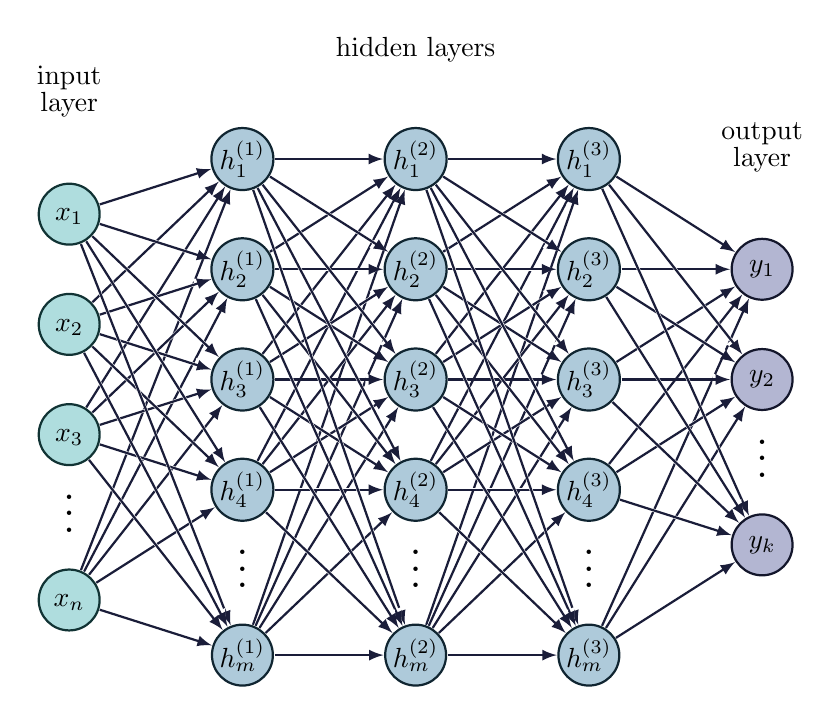
\begin{tikzpicture}[x=2.2cm,y=1.4cm]
      \readlist\Nnod{4,5,5,5,3}
      \readlist\Nstr{n,m,m,m,k}
      \readlist\Cstr{\strut x,h^{(\prev)},h^{(\prev)},h^{(\prev)},y} 
      \def\yshift{0.5} 
      % \message{^^J  Layer}
      \foreachitem \N \in \Nnod{ % loop over layers
        \def\lay{\Ncnt} % alias of index of current layer
        \pgfmathsetmacro\prev{int(\Ncnt-1)} % number of previous layer
        \message{\lay,}
        \foreach \i [evaluate={\c=int(\i==\N); \y=\N/2-\i-\c*\yshift;
                     \index=(\i<\N?int(\i):"\Nstr[\lay]");
                     \x=\lay; \n=\nstyle;}] in {1,...,\N}{ % loop over nodes
          % NODES
          \node[node \n] (N\lay-\i) at (\x,\y) {$\Cstr[\lay]_{\index}$};
          
          % CONNECTIONS
          \ifnum\lay>1 % connect to previous layer
            \foreach \j in {1,...,\Nnod[\prev]}{ % loop over nodes in previous layer
              \draw[connect,white,line width=1.2] (N\prev-\j) -- (N\lay-\i);
              \draw[->,connect] (N\prev-\j) -- (N\lay-\i);
              %\draw[connect] (N\prev-\j.0) -- (N\lay-\i.180); % connect to left
            }
          \fi % else: nothing to connect first layer
          
        }
        \path (N\lay-\N) --++ (0,1+\yshift) node[midway,scale=1.5] {$\vdots$};
      }
      
      % LABELS
      \node[above=0.5,align=center,black] at (N1-1.90) {input\\[-0.2em]layer};
      \node[above=0.5,align=center,black] at (N3-1.90) {hidden layers};
      \node[above=0.5,align=center,black] at (N\Nnodlen-1.90) {output\\[-0.2em]layer};
    \end{tikzpicture}}
    %\includegraphics[width=0.5\linewidth]{}
    \caption{Illustration of a feed-forward neural network with one input layer, three hidden layers, and one output layer, where $n$, $m$ and $k$ indicate the number of neurons in the respective layer.}
    \label{fig:ffnn}
\end{figure}
The architecture of a neural network is often determined by the problem to be solved. According to the universal approximation theorem, a FFNN with a minimum of one input layer, one hidden layer with a non-linear activation function, and one linear output layer, is sufficient to approximate a continuous function \cite[194]{Goodfellow:2016:deep_learning}. 

The output of a hidden layer can be written as 
\begin{equation}\label{eq:ffnn}
    \mathbf{h} = a \Big( \mathbf{W}^{T} \mathbf{x} + \mathbf{b} \Big) ,
\end{equation}
where $a$ is a non-linear activation function, $\mathbf{W}$ is the weight matrix, $\mathbf{x}$ is input, and $\mathbf{b}$ is the bias. 

\subsubsection{Weights and biases}\label{sssec:weights_biases}
The technique used to initialize the weights and biases in the FFNN can be vital for how fast the network learns. For a less ideal method, the network may need more iterations to find an optimal solution. Whereas a clever initialization may reduce the number of iteration needed, as the weight are some of the hyper-parameters that needs tuning. 

\subsubsection{Activation functions}\label{sssec:activation_functions}

Activation functions in neural networks are meant to represent neuronal firing, a process which in simplified terms is either on or off. Thus, the output 
of an activation function is going to be between 0 and 1, depending on the input. If 0, the neuron can be considered "dead" and will not contribute 
to the final prediction. If 1, the neuron is completely "on" and will pass on the information to the next node as described in Eq. (\cite{ffnn}). 

Here we separate between sigmoidal nonlinearities and rectified linear hidden units (ReLU). The latter is shown to give better results in many cases 
\cite{relu_best_ever}, but is not suitable as the final layer activation function. Sigmoidal nonlinear activation functions have been shown to 
cause vanishing gradients, as discussed in \ref{subsec:backpropagation}, but they are the golden standard as the final activation function. 
\\
\\
In our network, we choose between four different activation functions as presented below: 
\\
\\
1. \textbf{Sigmoid:}
The sigmoidal or logistic activation function is a saturating function that was previously used for all layers in early neural networks, 
however it's now more common as the final activation layer in binary classification networks.
\[
\sigma(z) = \frac{1}{1 + e^{-z}}
\]
\\
\\
2. \textbf{Softmax (for matrix input):}
The softmax activation functions has the same use-case as the sigmoidal, but for non-binary classification cases. 

For a matrix \( z \) with rows representing sets of scores, the softmax function can be applied to each row \( z_{i,:} \) as:
\[
\text{softmax}(z_{i,j}) = \frac{e^{z_{i,j} - \max(z_{i,:})}}{\sum_{k} e^{z_{i,k} - \max(z_{i,:})}}
\]
where \( \max(z_{i,:}) \) is the maximum value in the \( i \)-th row.
\\
\\
3. \textbf{ReLU (Rectified Linear Unit):}
The ReLU activation function is a simple non-saturating activation function that is useful to prevent gradients from vanishing during backpropagation, 
but it can also suffer from dead neurons when the output is 0, which makes it hard to update the weights during backpropagation.  
\[
\text{ReLU}(z) = 
\begin{cases} 
   z & \text{if } z > 0 \\
   0 & \text{otherwise}
\end{cases}
\]
\\
4. \textbf{Leaky ReLU:}
The leaky ReLU is a version of the ReLU above which was developed by A.L.Maas, A.Y.Hannum and A.Y.Ng \cite{relu_best_ever}. The $\delta$ coefficient avoids
setting each neuron to an absolute 0, which dealss the issue of dead neurons during backpropagation.
\[
\text{Leaky\_ReLU}(z) = 
\begin{cases} 
   z & \text{if } z > 0 \\
   \delta \cdot z & \text{otherwise}
\end{cases}
\]


\subsubsection{Loss functions}\label{sssec:loss_functions}
Loss functions in neural networks are key to training the weights and biases in a network, as they are the initial function we aim to minimize. 
Since the whole backpropagation step is essentially built around the derivative of our loss function, we provide a short summary of our choice of 
loss functions and where we've applied them. 
\\
\\
1. \textbf{Mean Squared Error (MSE):}
We use the mean square error as the loss function in all of our regression cases to compare how the targets differ from the predictions, such
as with the Topographical data preditions. 
   \[
   \text{MSE}(\hat{y}, y) = \frac{1}{n} \sum_{i=1}^{n} (\hat{y}_i - y_i)^2
   \]
   where:
   - \( \hat{y} \) are the predicted values.
   - \( y \) are the target values.
   - \( n \) is the number of data points.
\\
\\
2. \textbf{Cross-Entropy:}
We use cross-entropy (CE) as the loss function for all classification cases with more than two outcomes (non-binary). Although none of our results include
details on this, the ANN was tested on the Iris dataset with a cross-entropy loss function. 
   \[
   \text{CE}(\hat{y}, y) = -\sum_{i=1}^{n} y_i \log(\hat{y}_i)
   \]
   where \( y \) is the target and \( \hat{y} \) is the prediction .
   %
\\
\\
3. \textbf{Binary Cross-Entropy:}
We use binary cross entropy (bce) as the loss function for all binary classification cases, such as the Wisconsin Breast Cancer predictions. 
   \[
   \text{BCE}(\hat{y}, y) = -\frac{1}{n} \sum_{i=1}^{n} \left( y_i \log(\hat{y}_i) + (1 - y_i) \log(1 - \hat{y}_i) \right)
   \]
%
where \( y \) is the binary target and \( \hat{y} \) is the predicted probability.
\\

\subsubsection{Forward propagation}\label{sssec:forward_propagation}

\subsubsection{Back-propagation}\label{sssec:backpropagation}

Something about vanishing gradients...


%------------ Data --------------------------------------------
\subsection{Data}\label{ssec:data}
%
\paragraph*{Topographical data}
We obtained geographical data of the Stavanger area, Norway, from EarthExplorer (\footnote{\url{https://earthexplorer.usgs.gov/}}, 
via \footnote{\url{https://github.com/CompPhysics/MachineLearning/tree/master/doc/Projects/2023/Project1/DataFiles}}). 
The data contained a 200x200 grid of altitudes (m) of the area, with arbitrary x- and y-coordinates that we used as our features. 
We constructed a design matrix with polynomial features in the same manner as with synthetic data, and split the data in 80:20 training 
and data set using \texttt{train\_test\_split}. We scaled the data by standard normalization. We chose to scale since some linear regression 
models such as Lasso and Ridge perform better when all features are on a similar scale \supercite{raschka2019}. 
\\
\paragraph*{Wisconsin breast cancer data}
The Wisconsin data set \cite{bc_wisconsin} is considered to be a benchmark data set for testing novel or existing machine learning methods on, and 
there is extensive documentation on previously explored machine learning methods on the data that can be found here: 
\cite{wisconsin_example1}, \cite{wisconsin_example2} and \cite{wisconsin_example3}.

As described in the original article which produced the data \cite{first_wisconsin}, it consists of a 30 features describing biopsied cell nuclei from 
a total of 569 samples. To produce the data, non-invasive fine needle aspirations of tumors were put on glass and stained, 
then pictures were taken of each sample. The features were then derived from each image with a "computer diagnostic system" that 
analyzed the images and computed an extensive set of nuclei features such as radius, perimeter, area, smoothness, concavity, symmetry and texture. 

The authors Nick Street and William H. Wolberg from the original paper performed a classification using a variant on the Multisurface 
Method, where they reached an accuracy of 97$\%$ after a ten-fold cross validation process with a sensitivity of 0.9 and a specificity of 0.86. 
These terms are important to include in any analysis on medicinal data as the implementation of computer aided diagnosis in clinical practice 
needs to be thoughourly documented and understood by physicians beforehand. Sensitivity is described as $\frac{correct\ positive}{total\ positive}$, 
while the specificity is $\frac{correct\ negative}{total\ negative}$
%
%------------ Tools -------------------------------------------
\subsection{Tools}\label{ssec:tools}
The models were implemented in \verb|Python| version 3.12, and the figures produced using the \verb|matplotlib| library, and stylized using \verb|seaborn|. The FFNN was implemented from scratch, using the \verb|autograd| library \cite{maclaurin2015:autograd} for computing the gradients.
%================================================================
\section{Results}\label{sec:results}
% Present results and give a critical discussion of my work in 
% the context of other work. Relate the work to previous studies, 
% and make sure the results are reproducible. Include information 
% in figure captions such that they can give the reader enough to 
% understand the main gist of the report.
%================================================================

\subsection{Gradient descent}

We applied the gradient descent algorithm to data simulated from a third-degree polynomial without noise to assess convergence to the true parameters (APPENDIX). All parameters converged after approximately 800 iterations using plain gradient descent (figure \ref{fig:poly-converge}). Adding momentum to the gradient descent sped up convergence to around 4-fold (figure \ref{fig:poly-converge-momentum}), and using any optimizer had similar effects on convergence times (APPENDIX FIGS).

\begin{figure}
    \centering
    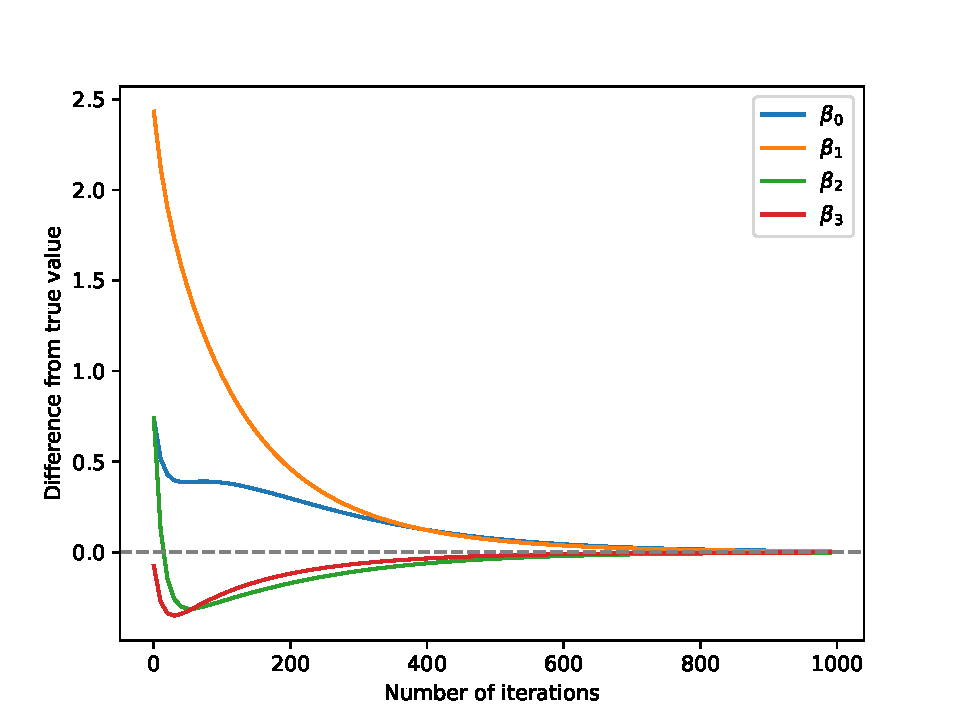
\includegraphics[width=0.99\linewidth]{examples/tests_even/figs/gradient-descent-polynomial-convergence.pdf}
    \caption{Gradient descent on data generated from a 4th degree polynomial without noise, using polynomial features up to the 4th degree. The stippled line represents 0 difference from the parameters used to generate the data.}
    \label{fig:poly-converge}
\end{figure}

\begin{figure}
    \centering
    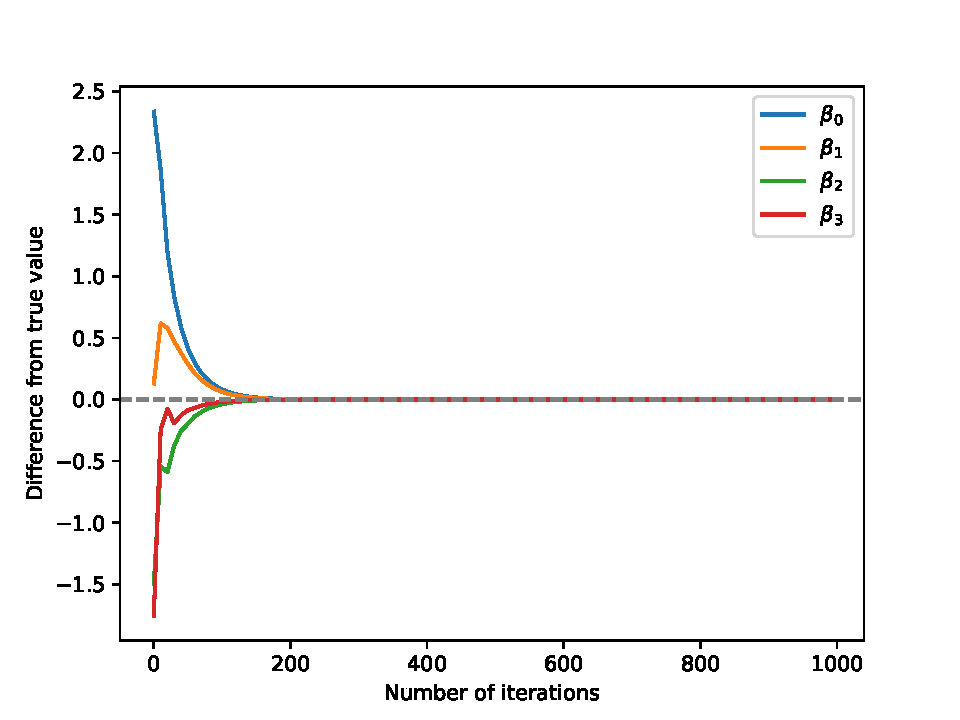
\includegraphics[width=0.99\linewidth]{examples/tests_even/figs/gradient-descent-momentum-polynomial-convergence.pdf}
    \caption{Gradient descent on the same data as in Figure \ref{fig:poly-converge}, but using momentum. The algorithm converged considerably faster than gradient descent without momentum.}
    \label{fig:poly-converge-momentum}
\end{figure}

The choice of learning rate affected the performance of the model regardless of optimizer. For data generated from the Franke function \cite{franke1979} with added noise, the different optimizers had different optimal learning rates, but in general a learning rate between $10^{-3}$ and $1$ gave the best results (figure \ref{fig:franke-learningrate}). For this particular data GD outperformed SGD (APPENDIX). Overall, ADAM consistently gave the lowest mean squared error on the test data over the largest range of learning rates. Because of this, we chose to emphasize ADAM over the other optimizers when analyzing the terrain data.

\begin{figure}
    \centering
    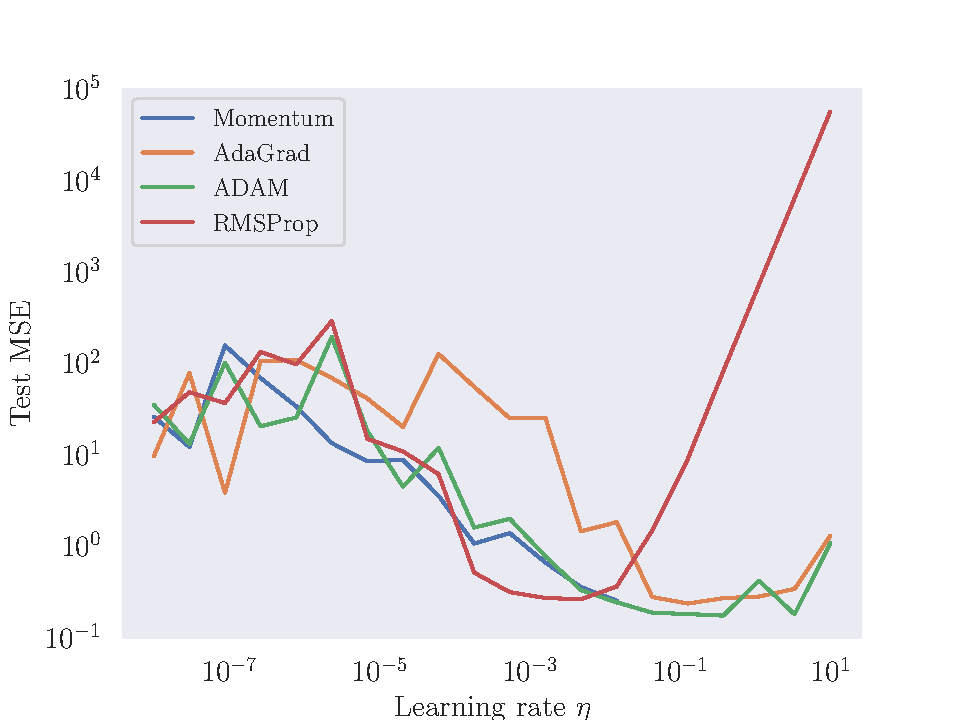
\includegraphics[width=0.99\linewidth]{examples/tests_even/figs/Franke-learningrates-optimizers.pdf}
    \caption{How learning rates affect the mean squared error in gradient descent with momentum or different optimizers. The data was generated from the Franke function, with added noise. For the momentum algorithm the gradient descent was not completed for learning rates above $10^{-2}$ due to exploding gradients.}
    \label{fig:franke-learningrate}
\end{figure}

For gradient descent on the terrain data ...

\begin{figure}
    \centering
    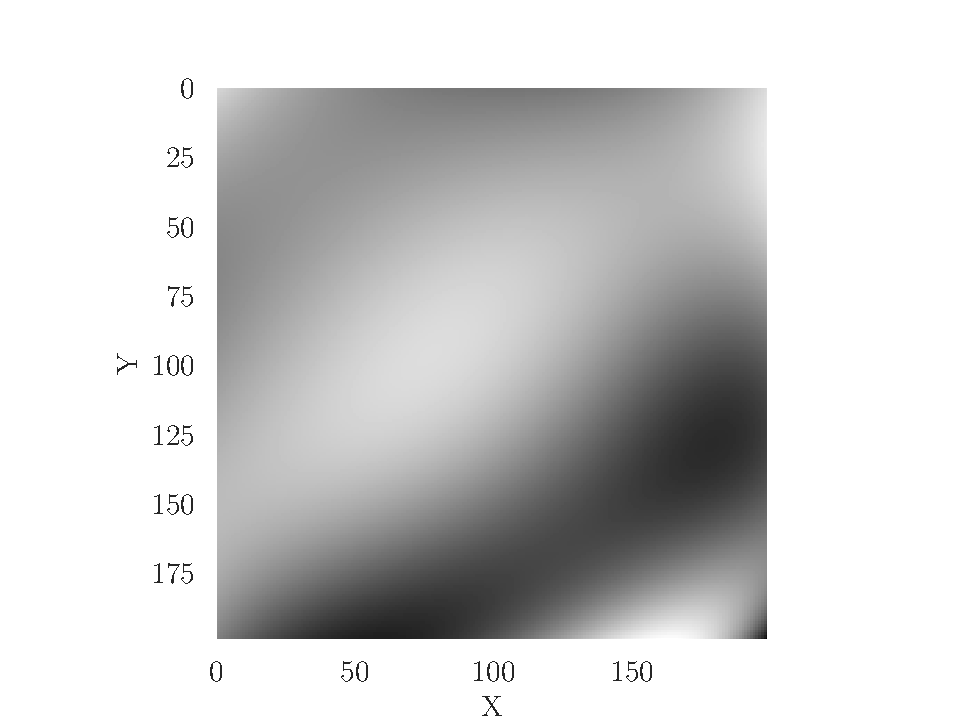
\includegraphics[width=0.99\linewidth]{examples/tests_even/figs/gradient-descent-terrain-map.pdf}
    \caption{Prediction of the terrain data from project 1 using gradient descent with a ridge gradient.}
    \label{fig:enter-label}
\end{figure}



- describe implementation\\
- Show all the different optimizers etc\\
- compare to regression from last project\\
- Based on this, we chose to keep this and this optimizer\\
- include figure of terrain, compare to ridge from last project and data\\



\subsection{Regression analysis with FFNN}

- compare to project 1\\
- discuss results compared to OLS/Ridge\\
- Optimal learning rates and parameters, lambda-learningrate grid-search\\
- discuss activation functions\\
- discuss initialization of learning rates\\


\subsection{Breast cancer data}
We tested a set of different optimizers and learning rates on our breast cancer (BC) data, and found the best optimizer to be Adam, as is the golden standard for many NN problems today. The optimal learning rate with Adam was 0.1. To perform the classification we chose two layers of size 100 and 2, where our final layer output was a $n x 2$ vector with probabilities. For information about this selection process, see our appendix. "cite something?"

After splitting and normalizing the input data, we trained our neural net against Sklearns MLPClassifier with the same amount of layers. We chose the ReLU6 activation function for the first 100-node layer, and the final layer was sigmoidal. For argumentation, see Subsection \ref{sssec:activation_functions}.

To prevent potential unwelcome batch effects that can occur from random splitting of test and train data, we did a 10-fold cross validation inside the NN-data and chose the back-propagation path with the best accuracy. The result was suprisingly that our neural network performed better than Sklearn to a very small degree, as presented below: 




- A couple of sentences on choosing optimizer
- Classification and accuracy of binary classification\\
- Discuss the results and analyze the different parameters used (learning rate, lambda) and the effect of different activation functions\\
- Compare with similar code from Scikit-Learn etc.\\
- Compare with logistic regression\\


%================================================================
\section{Conclusion}\label{sec:conclusion}
% State main findings and interpretations, and try to present 
% perspectives for future work. Discuss pros and cons of methodd, 
% and possible improvements.
%================================================================

Future works: 
- Dropout rate to prevent overfitting
- See if data could predict relapse (because relapse in bc is more deadly than the initial diagnosis)

Issues: 
- NN is a black box, diagnosticians need to understand how something works in order to use it in real life.
\newpage

 
%------------------ Bibliography --------------------------
\onecolumngrid
\newpage 
% \nocite{*}
\bibliography{references}

%------------------ Appendix ------------------------------
\newpage
\twocolumngrid
%================================================================
\appendix
% Additional calculations used to validate the codes, these 
% selected calculations can be listed with few comments. Can also 
% include listing of the code if you feel this is necessary
%================================================================

%------------------ Structure -----------------------------
% \tableofcontents 

%==========================================================
%------------------ End of project content ----------------
%==========================================================
\end{document}